% Seção 6: ar aprisionado (f100, alpha = 63,4 graus; confinamento, k_ra,min, malha)
\citet[pp.~1539, 1541]{rahardjo2007} conclude that slopes with $k_s\le10^{-6}$~m/s, ``even when the rainfall intensity
is extremely high'', do not fail under rainfalls of up to 24~h, because the rain does not raise the water table and
most of it runs off. We examine the $f_{100}$ soil ($k_s=3.6\mmh$) on the steepest slope of their study,
$\alpha=63.4^\circ$, whose initial FS is 1.775 in our analysis (Fig.~\ref{fig:ar}); their Fig.~9c gives about 1.69
for the initial FS and about 1.12 and 1.05 for the minimum FS with 9 and 80~mm/h (read from the figure). With the
usual model (iii) the minimum FS under 24-h rainfalls is 1.383, 1.163, 1.097 and 1.093 for $I_r=9$, 18, 36 and
80~mm/h: the slope does not fail, as \citet{rahardjo2007} conclude. With model (ii) the minimum FS is 0.015--0.041
higher. With active air (model i) it is 1.166, 1.028, 1.015 and 1.013: from 36~mm/h on, the minimum FS is within 0.02
of one at the end of the rainfall, i.e.\ the slope fails with $\delta=0.02$ ($I_{c,0.02}=29$~mm/h) but not with
$\delta=0.01$. With elements of 0.35~m near the surface the minimum FS with 36~mm/h is 1.009 (Section~\ref{sec:malha}).

\begin{figure}[htbp]
\centering
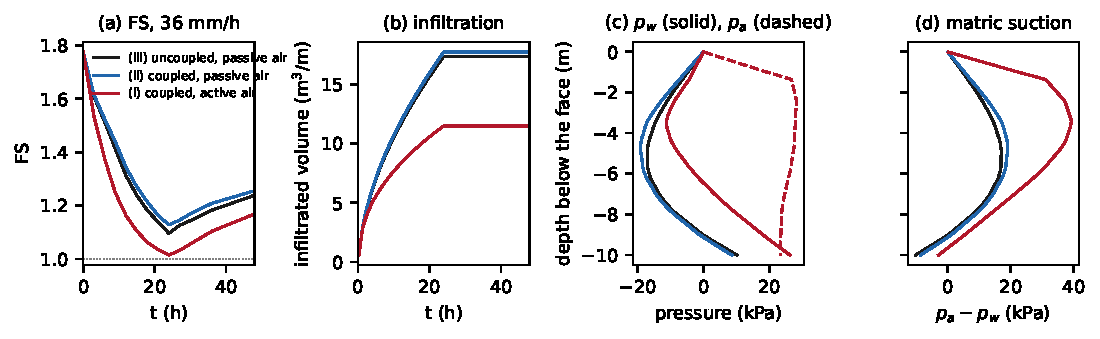
\includegraphics[width=\textwidth]{ar_aprisionado.pdf}
\caption{Soil $f_{100}$, $\alpha=63.4^\circ$, $I_r=36\mmh$ during 24~h, in models (i)--(iii). (a) FS; (b) infiltrated
volume; (c) water (solid) and air (dashed, model i) pressures and (d) matric suction along a vertical below the
middle of the face at $t=24$~h.}\label{fig:ar}
\end{figure}

The lower FS of model (i) is not associated with more water. With active air 10.4--11.6~m$^3$/m infiltrate in 24~h,
against 13.5--18.0~m$^3$/m with passive air (Fig.~\ref{fig:ar}b). The surface ponds earlier with active air: with
9~mm/h the first vertex ponds after 6~h with active air and after 11.75~h with passive air, and at the end of the
rainfall 83 and 41 of the 96 surface vertices are ponded; with 36~mm/h the whole surface ponds within 4.5~h with
active air and 6.5~h with passive air. With 36~mm/h the maximum air pressure is 19.5~kPa after 1~h, 30~kPa after 3~h
and 38~kPa after 24~h. At the end of the rainfall, along a vertical below the middle of the face
(Fig.~\ref{fig:ar}c,d), the air pressure averages 32~kPa between 0.5 and 5~m of depth; between 2 and 5~m the matric
suction is 38~kPa with active air and 24~kPa with passive air, and the water pressure is $-6\kpa$ with active air
and $-24\kpa$ with passive air. The matric suction is therefore higher with active air, while the water pressure,
which with $\chi=1$ is the only pressure in the effective stress (Eq.~\ref{eq:bishop}), is also higher. Across the
models, a smaller infiltrated volume comes with a smaller FS. \citet[p.~1539]{rahardjo2007} relate the decrease of
the minimum FS to the rainfall volume needed to initiate and to complete it; within each of our models the minimum FS
also decreases with the intensity, but between models with and without active air the ordering of volume and FS is
reversed.

The air pressure depends on how easily the air leaves through the ponded surface. With the minimum relative
permeability of the air $k_{ra}^{\min}$ between $10^{-6}$ and $10^{-3}$ the minimum FS is 1.013--1.015 and the maximum
air pressure 37--38~kPa; with $10^{-2}$ the air pressure falls to 28~kPa and the minimum FS rises to 1.046.

\subsection{Confinement of the air}\label{sec:confinamento}

The base and the lateral boundaries are closed to the air in the reference model. Opening them (atmospheric air
pressure on the base and on the lateral boundaries) changes the minimum FS by less than 0.002: 1.017 against 1.015 for
the $f_{100}$ slope with 36~mm/h, and 1.011 against 1.011 for the $f_{50}$ slope with 30~mm/h. The lateral boundaries
are 30~m away from the slope and the base is below the water table.

\subsection{Mesh}\label{sec:malha}

The minimum FS of the $f_{100}$ slope with 36~mm/h decreases with the mesh: 1.0154, 1.0122 and 1.0090 with elements
of 0.75, 0.5 and 0.35~m near the surface (1620, 3597 and 7314 triangles), by about 0.003 per refinement, while the
initial FS changes less at each refinement (1.775, 1.761 and 1.752; Fig.~\ref{fig:malha}). Whether the converged
minimum FS falls below one cannot be decided with these meshes.

\begin{figure}[htbp]
\centering
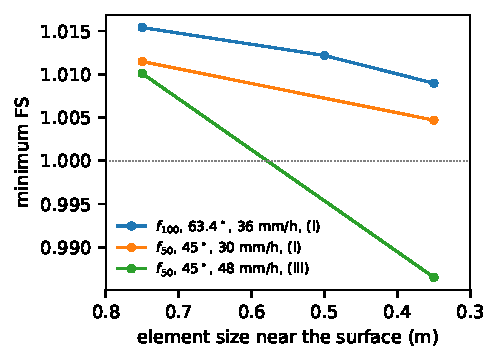
\includegraphics[width=0.5\textwidth]{malha.pdf}
\caption{Minimum FS against the element size near the surface: $f_{100}$ slope at $63.4^\circ$ with 36~mm/h in model
(i), and the $f_{50}$ reference slope near its critical intensities in models (i) and (iii).}\label{fig:malha}
\end{figure}
